% SHT21P kombineret temperatur- og fugtsensor

\begin{figure}[htb]
\centering
{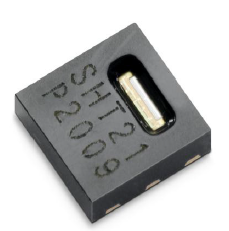
\includegraphics[width=0.25\textwidth]{filer/design/Billeder/sht21p_fysisk.png}}
\caption{Fysisk afbildning af SHT21P}
\label{lab:sht_filter}
\end{figure}

Til indsamling af temperatur- og fugtdata for golfhuller anvendes den kombineret temperatur og fugtsensor SHT21P. Denne er valgt ud fra at der således ikke behøves en sensor for hver af de to målinger, samt at denne giver et analog signal med i designet. SHT21P sender en PWM ud som midles til en DC-spænding med et 2. ordens lavpasfilter. Denne spændingen sendes ind i en A/D-convertor i PSoCen hvor denne behandles i en funktion, for så at returnere en temperatur eller fugt. Et select ben på SHT21P bestemmer hvorvidt denne måler temp. eller fugt. SCL HIGH(1) giver fugt output, SCL LOW(0) giver temperatur output.

\begin{figure}[htb]
\centering
{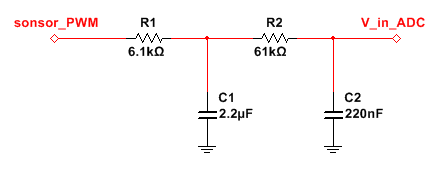
\includegraphics{filer/design/Billeder/sht21p_filter_pic.png}}
\caption{Multisim tegninger af 2. ordens filter}
\label{lab:sht_filter}
\end{figure}

Filterets knækfrekvens ($f_c$) er designet ud fra frekvensen på PWM signalet. Denne er opgivet til 120 Hz i databladet. Ved at designe filteret med en $f_c$ der ligger væsentligt under de 120 Hz, vil der opnås en stor dæmpning på amplituden således at signalet tilnærmer sig en fast DC-spænding svarende til middelværdien af PWM. PWMen oscillerer i området VSS-VDD. Sensoren er forsynet med 3,3 VDC og VSS er forbundet til GND, hvilket giver en PWM i området 0-3,3 VDC. Den nedre og ovre grænse for PWM er henholdsvis 10 \% og 90 \%, hvilket svarer til DC-værdierne 358 mV og 2790 mV.
\begin{equation}
f_c = \frac{1}{2 \pi * R1 * C1} = \frac{1}{2 \pi * 6,1*10^3  * 2,2*10^{-6}} = 11,86 Hz
\end{equation}
$f_c$ ligger således en dekade under de 120 Hz og da filteret er designet som et 2. ordens filter, vil det dæmpe 40 dB pr. dekade. Amplituden vil da være dæmpet ca. 6.7 gange og tilbage er den tilnærmet DC værdi. 

Grundet at værdien kun er tilnærmet skyldes at der stadig vil være en lille smule oscillation fra PWMen og støj.